\section{Unanswered questions about PT2+C}
\begin{frame}
    \frametitle{BW-PEOM(2)+C}
    \begin{figure}
        \centering
        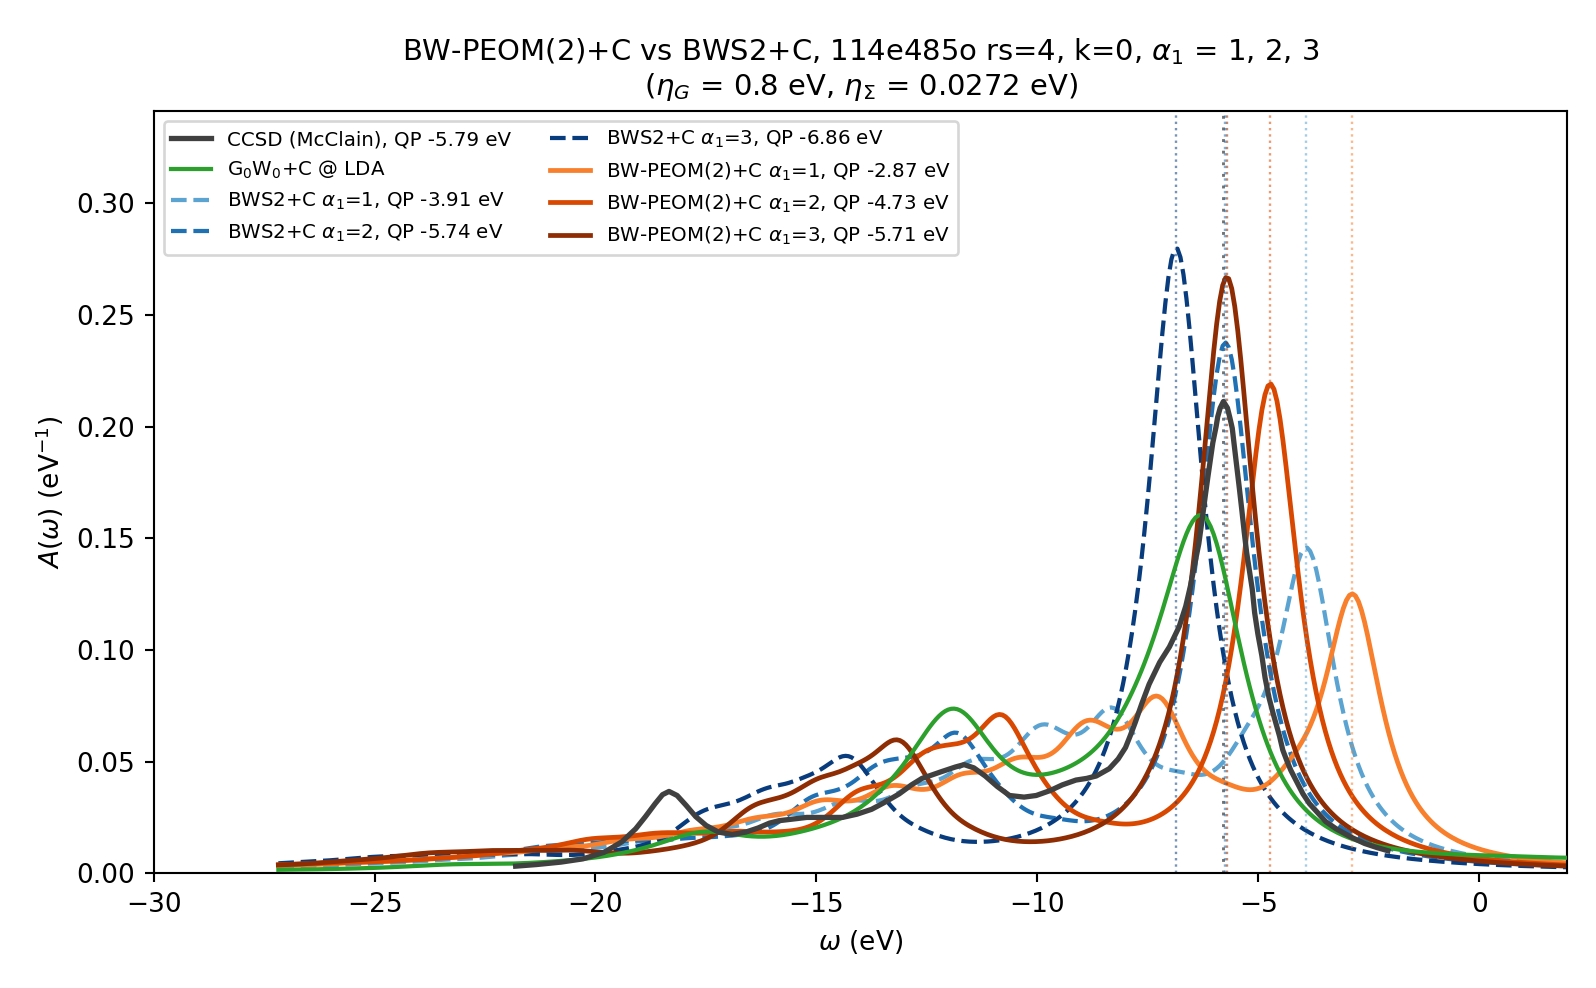
\includegraphics[width=\textwidth]{26/8/8-28/bw_peom_114e_joint_a11_2_3.png}
\end{figure}
\end{frame}
\begin{frame}
    \frametitle{BW-PEOM(2)+C cont.}
    \begin{figure}
        \centering
        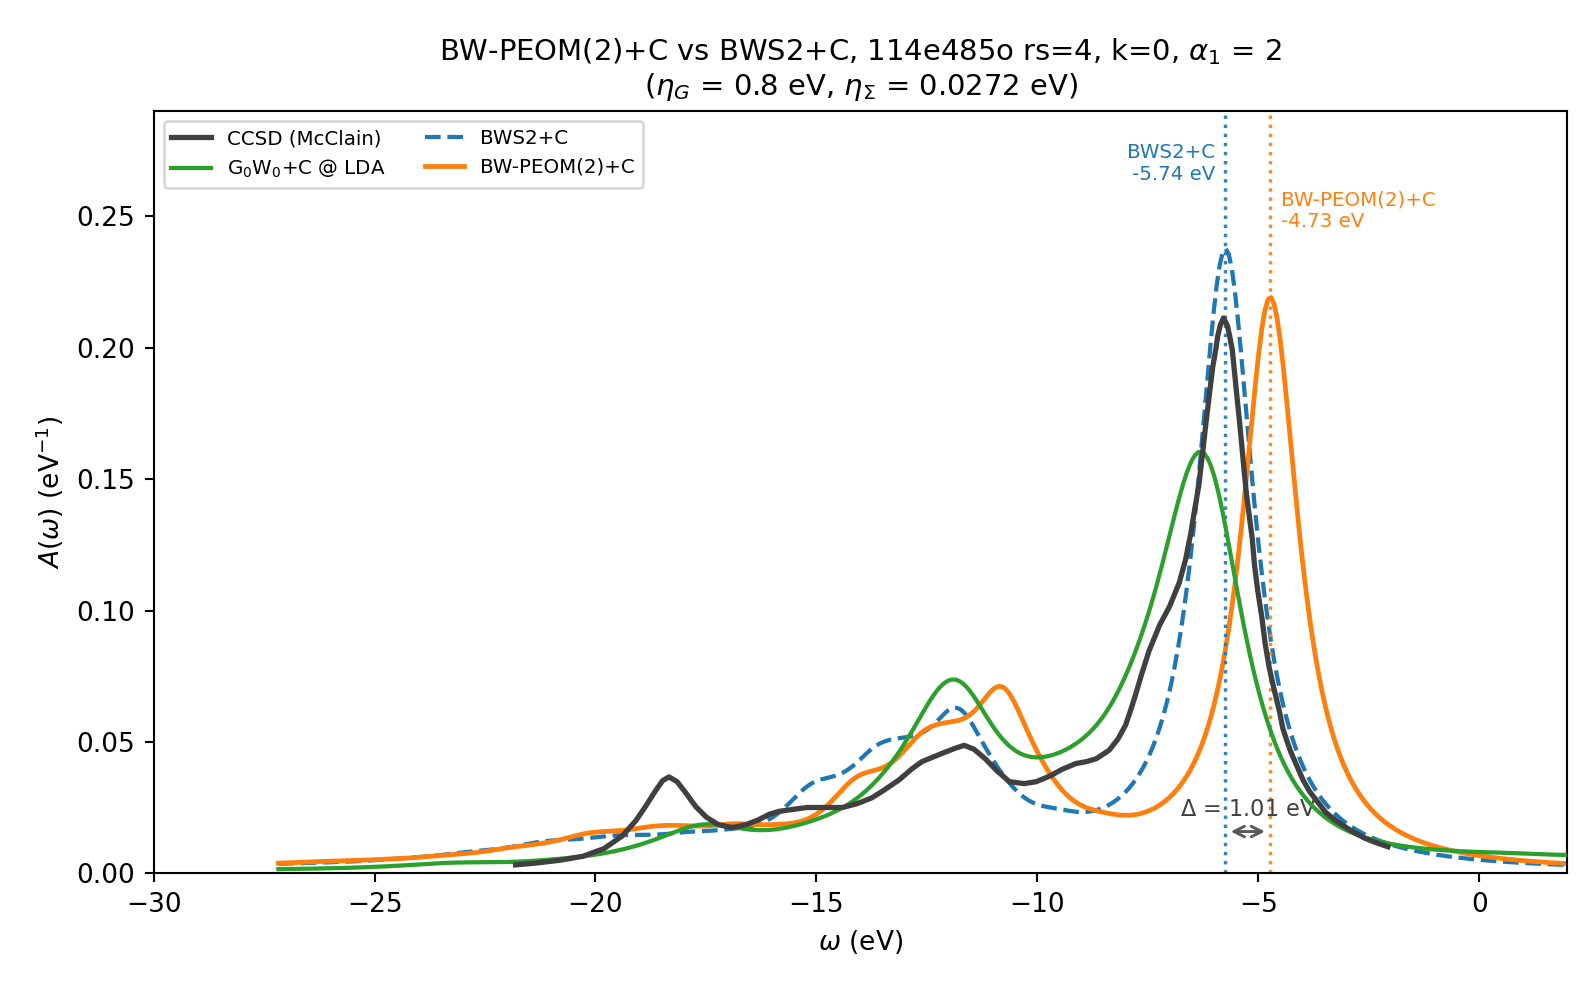
\includegraphics[width=\textwidth]{26/8/8-28/bw_peom_114e_joint_a12.png}
\end{figure}
\end{frame}
\begin{frame}
    \frametitle{Why doesn't this work}
Derivation of the Landau form relies upon 
\begin{align}
G_{pp}^{(0)'}(t)
C_{pp}^{\mathrm{BWs2}}(t)
&=
\int dt' dt'' \,
G_{pp}^{(0)'}(t - t')
\Sigma_{\mathrm{eff},pp}(t' - t'')
G_{pp}^{(0)'}(t''),
\end{align}
\pause
where we are equating the cumulant expansion to the Dyson equation to second order in $v$. \pause
\begin{itemize}
% \item To get $C^{(2)}$ in Landau form, we equate the cumulant expansion to the Dyson equation to second order in $v$. \pause
\item But PEOM(2) is known to incorporate third-order $v$ into $\Sigma$ \pause
\item This is what plagued our first attempt at SCCE via Dyson inversion
\end{itemize}
\begin{equation}
    \Sigma^R_{c,\text{Dyson}}(\omega) = \left[G_{c,0}^R(\omega)\right]^{-1} - \left[G^R_{c,\text{exact}}(\omega)\right]^{-1}
\end{equation}
\end{frame}
\begin{frame}
    \frametitle{Review of the available PT2+C methods}
Look at Nemo's IP/EA study on GW50
\end{frame}
\section{Self-consistent cumulants}

\begin{frame}
    \frametitle{SCCE(GW0) results}
    \begin{figure}
        \centering
        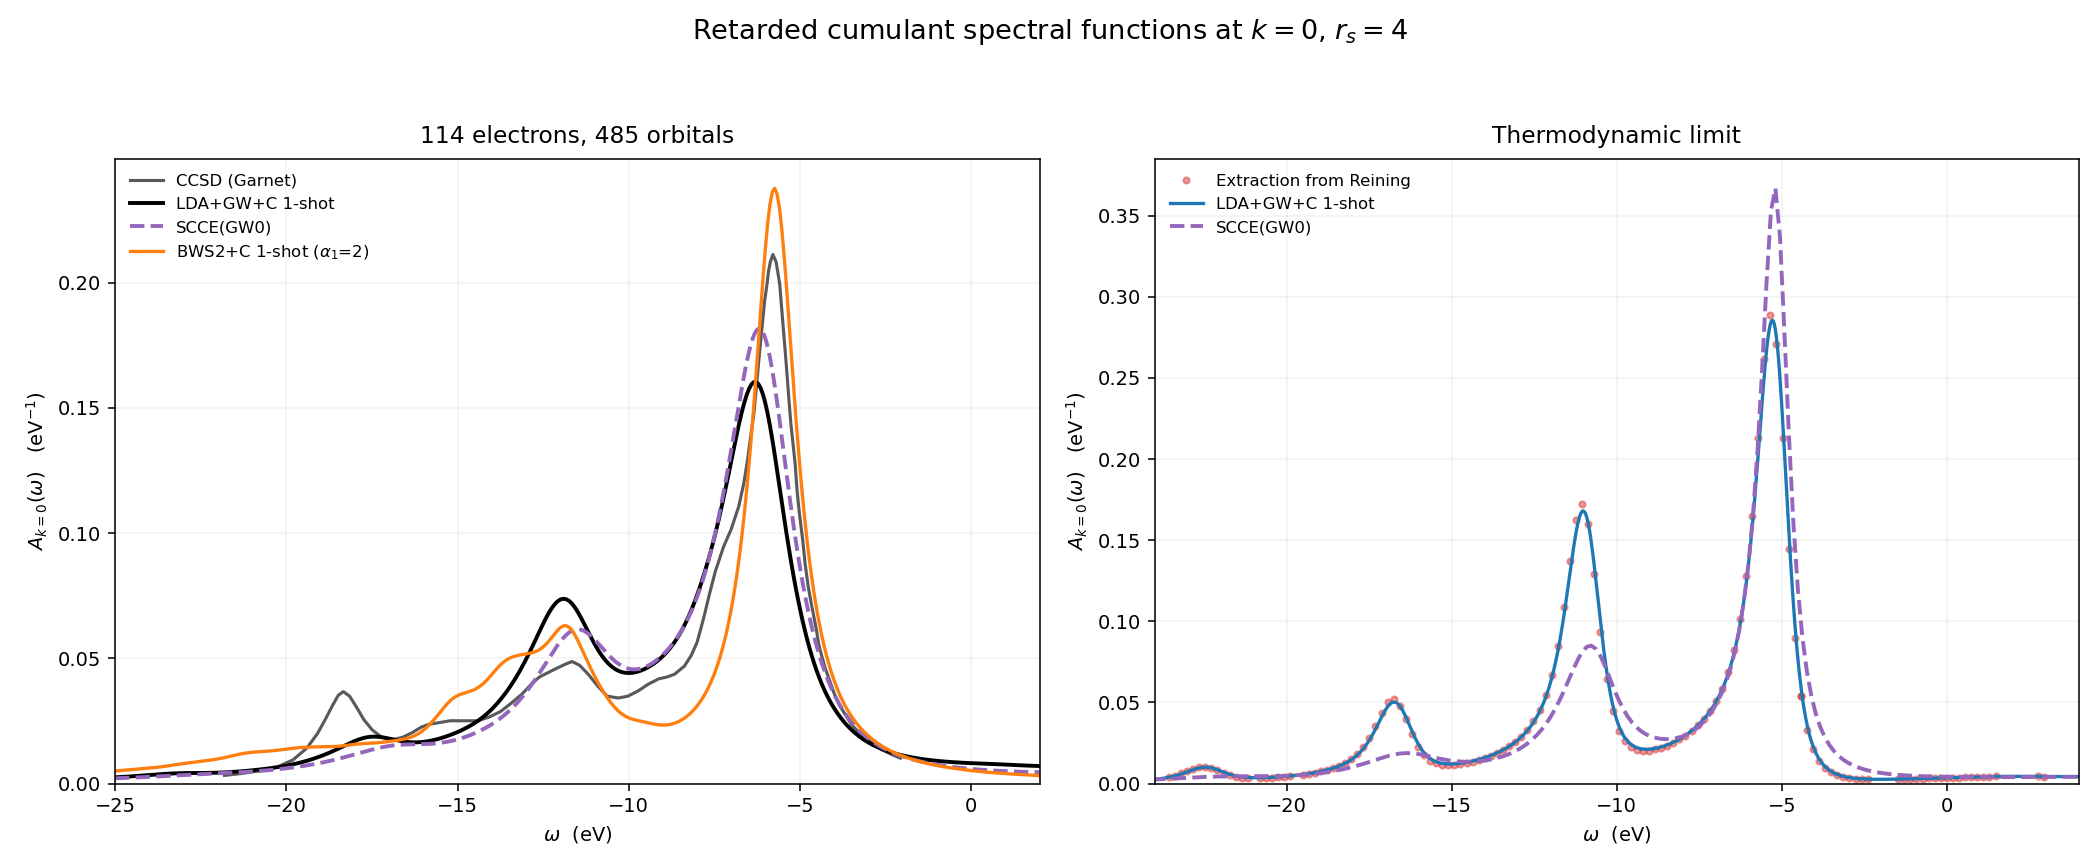
\includegraphics[width=\textwidth]{26/8/8-28/combined_k0_scce.png}
\end{figure}
\end{frame}
\begin{frame}
    \frametitle{SCCE(GW0) theory}
\begin{align} G^{n+1,R}_{k}(t) &= G_{0,k}^{n,R}(t) e^{C_{k}^{n+1,R}(t)}
\label{eq:cumulant_G}\end{align}
where $G_{0,k}^{n,R}(t) = -i \Theta(t) e^{-i \left(k^2/2 + \Gamma_k^{n}\right) t}$ with $\Gamma_k^{0} = V_k^{xc}$. \pause For $n\geq0$,
\begin{equation}
  \Gamma_k^{n+1} = n_{k}^{(n)}v_m+\Sigma_k^{n+1,x(E)}[G^{(n)}]=n_{k}^{(n)}v_m-\sum_{\bm{q}\neq\bm{0}} n_{\bm{k}+\bm{q}}^{(n)}v(\bm{q})  
\end{equation}\pause
After going through the algebra, we arrive at 
\begin{align}
G_k^{n+1,R}(t) &= - i\Theta(t)\, \exp\left[-i \left(k^2/2+\Gamma_k^{n+1}\right) t \right] e^{C_k^{n+1,\text{dyn}}(t)}.
\end{align}\pause
with
 \begin{align}
C_k^{n+1,\text{dyn}}(t) 
% &= \int d\omega\, \beta_{k}^{n+1,R}(\omega)\,\frac{e^{-i\omega t}-1}{\omega^{2}}\\
&= \underbrace{\int\!\dd\omega\,\beta_{k}^{n+1,R}(\omega)
    \frac{e^{-i\omega t}+i\omega t-1}{\omega^2}}_{C^{\rm Landau}_k(t)}
  \;-\; i\,S_1[\beta_k]\,t
\end{align}
where $\beta_{k}^{n+1,R}(\omega)=\frac{1}{\pi}\left|\operatorname{Im}\Sigma_k^{n+1,c}
\!\left(\omega+E_k^{(n)}\right)\right|$ \& $S_1[\beta_k]=\mathcal{P} \int\!\dd\omega\,\frac{\beta_{k}^{n+1,R}(\omega)}{\omega}$.
\end{frame}
\begin{frame}
    \frametitle{SCCE(GW0) cont.}
\begin{itemize}
\item Claude confirmed that TDL and finite basis SCCE(GW0) implementations are equivalent \pause
\item To confirm, I should converge to the TDL as I did with G0W0+C
\end{itemize}
    \begin{figure}
        \centering
        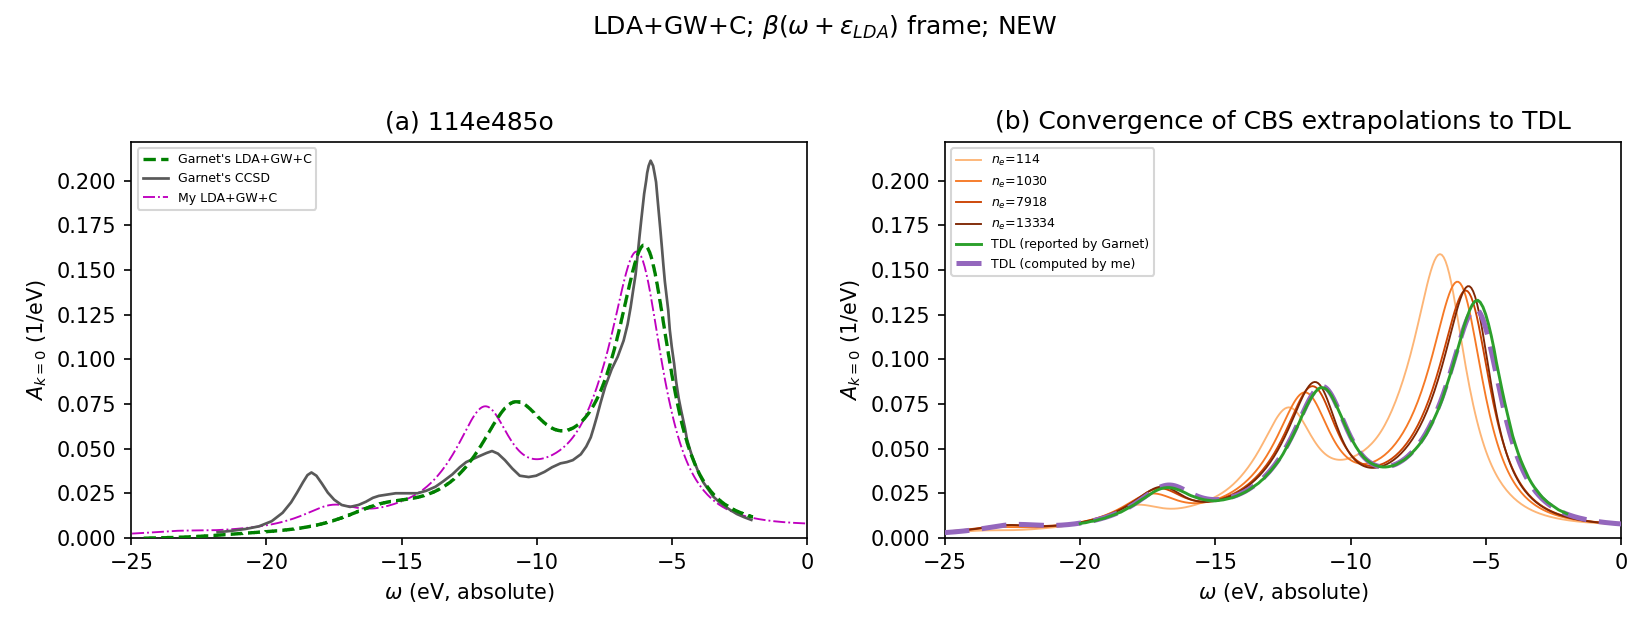
\includegraphics[width=\textwidth]{26/8/8-28/mcclain_gwc_compare_es0p0272.png}
\end{figure}
\end{frame}
\section{What to do next}
\begin{frame}
    \frametitle{Self-consistent cumulants}
\begin{itemize}
    \item Converge finite-basis SCCE(GW0) to the TDL in order to assert equivalence\pause
    \item Try to derive SCCE(G$\tilde{v}_0$) \pause
    \item Apply PJ's SCCE to the UEG?
\end{itemize}
\end{frame}

% \section{Get spectral functions for the UEG via dCC}
\begin{frame}
    \frametitle{Get spectral functions for the UEG via dCC}
Consider
\begin{equation}
H_p^{\rm el-pol}
=
\epsilon_p^{\rm MF} a_p^{\dagger} a_p
+
\sum_{m\nu}
\Delta_{pm\nu}
B_{pm\nu}^{\dagger}
B_{pm\nu}
+ a_p^{\dagger} a_p
\sum_{m\nu}
\left(
\mathcal{M}_{pm\nu}
B_{pm\nu}^{\dagger}
+
\mathcal{M}_{pm\nu}^{*}
B_{pm\nu}
\right),
\end{equation}
with QB operators $B_{pm\nu}^{\dagger}$. \pause
$\Delta_{pm\nu} = \epsilon_p^{\rm MF} - \epsilon_m^{\rm MF} + \operatorname{sgn}(\epsilon_m^{\rm MF} - \epsilon^{\rm MF}_{k_F})\Omega_\nu$ and $\mathcal{M}_{pm\nu}$ are QB excitation energies and couplings, respectively. \pause
This is the Hamiltonian for the electronic polaron in the QBA. \pause We used it to obtain Green's functions for GW+C and PT2+C. \pause It seems to me that in order to get Hamlin's dCC, instead of getting bosonic quantites from the QBA, one gets them with DFPT.
\end{frame}
